\chapter{Kinematika Titik}\label{ch:b1:point-kinematics}

Kereta pada sebuah kereta luncur memasuki loopnya pada \qty{90}{km/h},
melambat sambil menanjak, tergantung sesaat di puncaknya, lalu meraung
keluar lagi; penumpangnya merasa terhimpit ke kursinya di dasar dan
nyaris tanpa berat di puncaknya. Menggambarkan perjalanan itu --- di
mana keretanya, seberapa cepat ia bergerak, bagaimana \omterm{def:b1:point-kinematics:velocity}{kecepatannya}
berbelok dan berubah --- itulah kinematika, dan ia menuntut lebih
daripada $x$, $y$, $z$ sebuah jalan lurus: \omterm{def:b1:point-kinematics:cylindrical}{koordinat polar} untuk apa pun
yang berputar, dan kerangka yang ikut berjalan bersama keretanya
sendiri. Bab ini menyiapkan perkakas itu, membuktikan rumus \omterm{def:b1:point-kinematics:velocity}{kecepatan}
dan \omterm{def:b1:point-kinematics:velocity}{percepatan} pada masing-masingnya, lalu menerapkannya pada gerak yang
akan dipanggil setiap bab berikutnya: melingkar, heliks, harmonik, dan
gerak menyusuri sebarang kurva.

\section{Kedudukan, kecepatan, percepatan}

\begin{definition}[Kerangka acuan; kedudukan; lintasan]\label{def:b1:point-kinematics:frame}
\index{kerangka acuan}\index{vektor posisi}\index{lintasan}\index{partikel titik}
\emph{Kerangka acuan} adalah benda tegar yang dianggap tetap
(laboratorium, Bumi, sebuah kereta), bersama sebuah jam. \emph{Partikel
titik} $M$ --- benda yang ukurannya tak berarti bagi gerak yang
dipelajari --- ditentukan letaknya pada tiap saat oleh \emph{vektor
posisi}nya $\vect{OM}(t)$ dari titik asal $O$ yang melekat pada
kerangkanya; kurva yang digambarkan $M$ adalah \emph{lintasan}nya. Gerak
selalu berupa gerak \emph{relatif terhadap sebuah kerangka}: penumpang
yang sama diam di dalam keretanya dan bergerak di stasiunnya.
\end{definition}

\begin{definition}[Kecepatan dan percepatan]\label{def:b1:point-kinematics:velocity}
\index{kecepatan}\index{percepatan}
\emph{Kecepatan} dan \emph{percepatan} $M$ dalam kerangkanya adalah
\[
\vect v = \frac{\dd\vect{OM}}{\dd t}, \qquad
\vect a = \frac{\dd\vect v}{\dd t} = \frac{\dd^2\vect{OM}}{\dd t^2},
\]
yaitu turunan fungsi vektor: turunan sebuah vektor diperoleh dengan
menurunkan komponennya dalam basis yang \emph{tetap di dalam
kerangkanya}. Kecepatannya menyinggung \omterm{def:b1:point-kinematics:frame}{lintasannya} dan menunjuk searah
geraknya; normanya $v$ adalah \emph{kelajuan}nya. Satuannya:
\unit{m/s}, \unit{m/s^2}.
\end{definition}

\begin{proposition}[Koordinat Kartesius]\label{prop:b1:point-kinematics:cartesian}
\index{koordinat Kartesius}
Dengan basis ortonormal tetap $(\vect e_x, \vect e_y, \vect e_z)$ dan
$\vect{OM} = x\,\vect e_x + y\,\vect e_y + z\,\vect e_z$,
\[
\vect v = \dot x\,\vect e_x + \dot y\,\vect e_y + \dot z\,\vect e_z, \qquad
\vect a = \ddot x\,\vect e_x + \ddot y\,\vect e_y + \ddot z\,\vect e_z,
\]
dengan titik menyatakan $\dd/\dd t$.
\end{proposition}

\begin{proof}
Vektor basisnya tetap; hanya komponennya yang berubah.
\end{proof}

\begin{example}[Proyektil]\label{ex:b1:point-kinematics:projectile}
Ditembakkan dari $O$ dengan laju $v_0$ dan sudut $\alpha$ di atas
mendatar, koordinat sebuah bola (dinamika, bab berikutnya) adalah
$x = v_0\cos\alpha\,t$, $z = v_0\sin\alpha\,t - \tfrac12 gt^2$. Maka
$\vect v = v_0\cos\alpha\,\vect e_x + (v_0\sin\alpha - gt)\vect e_z$,
$\vect a = -g\vect e_z$: \omterm{def:b1:point-kinematics:velocity}{percepatannya} tetap sementara \omterm{def:b1:point-kinematics:velocity}{kecepatannya}
berbelok; di puncaknya ($\dot z = 0$, $t = v_0\sin\alpha/g$)
\omterm{def:b1:point-kinematics:velocity}{kecepatannya} mendatar dan \omterm{def:b1:point-kinematics:velocity}{percepatannya} tegak lurus terhadapnya. Dengan
menghilangkan $t$: $z = x\tan\alpha - gx^2/(2v_0^2\cos^2\alpha)$, sebuah
parabola.
\end{example}

\begin{omfigure}
\begin{tikzpicture}[font=\small, x=1cm, y=1cm]
  \draw[-Stealth] (0,0) -- (6.8,0) node[right] {$x$};
  \draw[-Stealth] (0,0) -- (0,3.6) node[above] {$z$};
  \node[below left] at (0,0) {$O$};
  \draw[omDef, thick, domain=0:6, samples=80] plot (\x, {2.2*\x - 0.3667*\x*\x});
  % point at x=1.5: z=2.2*1.5-0.3667*2.25=3.3-0.825=2.475 ; slope = 2.2 - 0.7333*1.5 = 1.1
  \fill[omThm] (1.5,2.475) circle (1.6pt); \node[above left] at (1.5,2.475) {$M$};
  \draw[-Stealth, omThm, thick] (1.5,2.475) -- ++(1.0,1.1) node[above right] {$\vect v$};
  \draw[-Stealth, omProp, thick] (1.5,2.475) -- ++(0,-1.2) node[right] {$\vect a = \vect g$};
  \draw[-Stealth, omExo] (0,0) -- (1.5,2.475); \node[omExo, left] at (0.72,1.45) {$\vect{OM}$};
  % apex at x=3: z=6.6-3.3=3.3
  \fill[omThm] (3,3.3) circle (1.6pt);
  \draw[-Stealth, omThm, thick] (3,3.3) -- ++(1.2,0);
  \draw[-Stealth, omProp, thick] (3,3.3) -- ++(0,-1.2);
\end{tikzpicture}

{\small Parabola sebuah proyektil: \omterm{def:b1:point-kinematics:velocity}{kecepatannya} menyinggung \omterm{def:b1:point-kinematics:frame}{lintasannya}
dan berbelok, sedangkan \omterm{def:b1:point-kinematics:velocity}{percepatan} $\vect g$ tetap. Di puncaknya
\omterm{def:b1:point-kinematics:velocity}{kecepatan} dan \omterm{def:b1:point-kinematics:velocity}{percepatannya} tegak lurus: kelajuannya sesaat stasioner
sementara arahnya masih berubah.}
\end{omfigure}

\section{Koordinat silinder}

\begin{definition}[Koordinat silinder dan basisnya]\label{def:b1:point-kinematics:cylindrical}
\index{koordinat silinder}\index{koordinat polar}\index{basis lokal}
Titik $M$ ditentukan letaknya oleh $r \geq 0$ (jaraknya ke sumbu $z$),
sudut $\theta$ proyeksinya pada bidang $xy$ terhadap $\vect e_x$,
dan $z$: $\vect{OM} = r\,\vect e_r + z\,\vect e_z$, dengan
\[
\vect e_r = \cos\theta\,\vect e_x + \sin\theta\,\vect e_y, \qquad
\vect e_\theta = -\sin\theta\,\vect e_x + \cos\theta\,\vect e_y,
\]
dan $\vect e_z$ membentuk \emph{basis lokal} $(\vect e_r, \vect e_\theta,
\vect e_z)$, yang ortonormal dan langsung, dan yang \emph{bergerak
bersama $M$}. Pada bidangnya ($z$ tetap) inilah \emph{koordinat polar}
$(r, \theta)$.
\end{definition}

\begin{lemma}[Turunan basis lokalnya]\label{lem:b1:point-kinematics:basisderiv}
\[
\frac{\dd\vect e_r}{\dd t} = \dot\theta\,\vect e_\theta, \qquad
\frac{\dd\vect e_\theta}{\dd t} = -\dot\theta\,\vect e_r, \qquad
\frac{\dd\vect e_z}{\dd t} = \vect 0 .
\]
\end{lemma}

\begin{proof}
Turunkan komponennya: $\dd\vect e_r/\dd t = \dot\theta(-\sin\theta\,
\vect e_x + \cos\theta\,\vect e_y) = \dot\theta\vect e_\theta$, dan
serupa untuk $\vect e_\theta$. Turunan sebuah vektor satuan yang
berputar tegak lurus terhadapnya, dengan norma sebesar laju sudutnya.
\end{proof}

\begin{theorem}[Kecepatan dan percepatan dalam koordinat silinder]\label{thm:b1:point-kinematics:cylindrical}
\[
\vect v = \dot r\,\vect e_r + r\dot\theta\,\vect e_\theta + \dot z\,\vect e_z,
\qquad
\vect a = \big(\ddot r - r\dot\theta^2\big)\vect e_r
+ \big(r\ddot\theta + 2\dot r\dot\theta\big)\vect e_\theta + \ddot z\,\vect e_z .
\]
\end{theorem}

\begin{proof}
Turunkan $\vect{OM} = r\vect e_r + z\vect e_z$ dengan lemanya:
$\vect v = \dot r\vect e_r + r\dot\theta\vect e_\theta + \dot z\vect e_z$.
Turunkan sekali lagi: $\ddot r\vect e_r + \dot r\dot\theta\vect e_\theta +
\dot r\dot\theta\vect e_\theta + r\ddot\theta\vect e_\theta - r\dot\theta^2
\vect e_r + \ddot z\vect e_z$; lalu kumpulkan.
\end{proof}

\begin{omfigure}
\begin{tikzpicture}[font=\small, x=1cm, y=1cm]
  \draw[-Stealth] (0,0) -- (5.2,0) node[right] {$x$};
  \draw[-Stealth] (0,0) -- (0,3.6) node[above] {$y$};
  \node[below left] at (0,0) {$O$};
  \coordinate (M) at (35:3.4);
  \draw[omExo] (0,0) -- (M); \fill[omThm] (M) circle (1.6pt); \node[below right, xshift=2pt] at (M) {$M$};
  \node[omExo] at (20:1.9) {$r$};
  \draw (0.9,0) arc (0:35:0.9); \node at (17:1.15) {$\theta$};
  \draw[-Stealth, omDef, very thick] (M) -- ++(35:1.1) node[right] {$\vect e_r$};
  \draw[-Stealth, omDef, very thick] (M) -- ++(125:1.0) node[left] {$\vect e_\theta$};
  % trajectory sketch: spiral
  \draw[omThm, thick, domain=5:75, samples=50, variable=\t] plot ({(2.2+0.0343*\t)*cos(\t)},{(2.2+0.0343*\t)*sin(\t)});
  \draw[-Stealth, omThm, thick] (M) -- ++(100:1.6) node[above right] {$\vect v$};
\end{tikzpicture}

{\small \omterm{def:b1:point-kinematics:cylindrical}{Koordinat polar}: \omterm{def:b1:point-kinematics:cylindrical}{basis lokalnya} $(\vect e_r, \vect e_\theta)$
berputar bersama $M$; \omterm{def:b1:point-kinematics:velocity}{kecepatannya} mempunyai bagian radial $\dot r$ dan
bagian ortoradial $r\dot\theta$. Di sini \omterm{def:b1:point-kinematics:frame}{lintasannya} (merah) memilin ke
luar, sehingga $\dot r > 0$ dan $\vect v$ condong ke luar dari garis
singgung lingkarannya.}
\end{omfigure}

\begin{corollary}[Gerak melingkar]\label{cor:b1:point-kinematics:circular}
\index{gerak melingkar}\index{percepatan sentripetal}\index{kecepatan sudut}
Pada lingkaran berjari-jari $R$ ($r = R$, $z = 0$), dengan
\emph{\omterm{cor:b1:point-kinematics:circular}{kecepatan sudut}} $\omega = \dot\theta$:
\[
\vect v = R\omega\,\vect e_\theta, \qquad
\vect a = -R\omega^2\,\vect e_r + R\dot\omega\,\vect e_\theta
= -\frac{v^2}{R}\,\vect e_r + \frac{\dd v}{\dd t}\,\vect e_\theta .
\]
Untuk \omterm{cor:b1:point-kinematics:circular}{gerak melingkar} \emph{beraturan} ($\omega$ tetap), \omterm{def:b1:point-kinematics:velocity}{percepatannya}
murni \emph{sentripetal}, bernorma $v^2/R = R\omega^2$, walaupun
kelajuannya tetap.
\end{corollary}

\begin{proof}
Tetapkan $\dot r = \ddot r = 0$ dalam teoremanya; $v = R\omega$.
\end{proof}

\begin{example}[Dua lingkaran]\label{ex:b1:point-kinematics:circles}
Sebuah mobil memutari bundaran berjari-jari \qty{20}{m} pada
\qty{36}{km/h} (\qty{10}{m/s}): $a = v^2/R = \qty{5.0}{m/s^2}$, separuh
$g$, terarah ke pusatnya --- itulah yang harus dipasok bannya. Bulan
($R = \qty{3.84e8}{m}$, $T = \qty{27.3}{d}$): $\omega = 2\pi/T =
\qty{2.66e-6}{rad/s}$, $a = R\omega^2 = \qty{2.7e-3}{m/s^2}$, seper
$3600$ dari $g$ di permukaan Bumi, pada enam puluh jari-jari Bumi ---
perbandingan yang dibuat Newton (\cref{ch:b1:central-forces}).
\end{example}

\section{Koordinat bola}

\begin{definition}[Koordinat bola]\label{def:b1:point-kinematics:spherical}
\index{koordinat bola}
Titik $M$ ditentukan letaknya oleh jaraknya $r = OM$, \emph{kolatitude}
$\theta \in [0, \pi]$ antara $\vect{OM}$ dan $\vect e_z$, serta
\emph{azimut} $\varphi$ proyeksinya pada bidang $xy$:
$\vect{OM} = r\,\vect e_r$ dengan
\[
\vect e_r = \sin\theta\cos\varphi\,\vect e_x + \sin\theta\sin\varphi\,\vect e_y + \cos\theta\,\vect e_z ;
\]
$\vect e_\theta$ (menyinggung meridiannya, ke arah $\theta$ yang menaik)
dan $\vect e_\varphi$ (menyinggung lingkaran lintangnya) melengkapi
basis ortonormal lokalnya. Di Bumi, $\theta$ adalah $90^\circ$ dikurangi
lintangnya dan $\varphi$ adalah bujurnya.
\end{definition}

\begin{proposition}[Kecepatan dalam koordinat bola]\label{prop:b1:point-kinematics:sphericalv}
\[
\vect v = \dot r\,\vect e_r + r\dot\theta\,\vect e_\theta + r\sin\theta\,\dot\varphi\,\vect e_\varphi .
\]
\end{proposition}

\begin{proof}
$\dd\vect e_r/\dd t = \dot\theta\,\vect e_\theta + \sin\theta\,\dot\varphi\,
\vect e_\varphi$: suku pertamanya adalah perputaran pada bidang
meridiannya (seperti pada kasus polarnya), suku keduanya perputaran
terhadap $\vect e_z$ dengan laju $\dot\varphi$ sebuah vektor yang
jaraknya ke sumbunya adalah $\sin\theta$. Lalu
$\vect v = \dd(r\vect e_r)/\dd t$. \omterm{def:b1:point-kinematics:velocity}{Percepatannya} tak diperlukan tahun ini.
\end{proof}

\begin{omfigure}
\begin{tikzpicture}[font=\small, x=1cm, y=1cm, scale=0.95]
  \draw[-Stealth] (0,0) -- (-2.4,-0.96) node[below left] {$x$};
  \draw[-Stealth] (0,0) -- (4.2,0) node[right] {$y$};
  \draw[-Stealth] (0,0) -- (0,3.6) node[above] {$z$};
  \node[below right] at (0,0) {$O$};
  \coordinate (M) at (1.4,2.4);
  \coordinate (P) at (1.4,-0.3);
  \draw[omExo] (0,0) -- (M); \fill[omThm] (M) circle (1.6pt); \node[above left] at (M) {$M$};
  \draw[dashed] (M) -- (P); \draw[dashed] (0,0) -- (P);
  \node[omExo] at (0.45,1.45) {$r$};
  \draw (0,1.0) arc (90:60:1.0); \node at (0.3,1.25) {$\theta$};
  \draw (-0.74,-0.3) arc (202:348:0.8); \node at (0.15,-1.05) {$\varphi$};
  \draw[-Stealth, omDef, very thick] (M) -- ++(0.45,0.77) node[above] {$\vect e_r$};
  \draw[-Stealth, omDef, very thick] (M) -- ++(0.77,-0.45) node[right] {$\vect e_\theta$};
  \draw[-Stealth, omDef, very thick] (M) -- ++(0.84,0.33) node[right] {$\vect e_\varphi$};
\end{tikzpicture}

{\small \omterm{def:b1:point-kinematics:spherical}{Koordinat bola} $(r, \theta, \varphi)$ dan \omterm{def:b1:point-kinematics:cylindrical}{basis lokalnya}:
$\vect e_r$ radial, $\vect e_\theta$ menyusuri meridiannya (ke arah
selatan pada sebuah bola dunia), $\vect e_\varphi$ menyusuri lingkaran
lintangnya (ke arah timur).}
\end{omfigure}

\section{Basis Frenet}

\begin{definition}[Absis lengkung; basis Frenet]\label{def:b1:point-kinematics:frenet}
\index{absis lengkung}\index{basis Frenet}\index{jari-jari kelengkungan}
Sepanjang sebuah \omterm{def:b1:point-kinematics:frame}{lintasan}, \emph{absis lengkung} $s(t)$ adalah panjang
busur dari sebuah titik acuan, yang dihitung secara aljabar; $v = \dot s$.
Di $M$, vektor singgung satuan $\vect T = \dd\vect{OM}/\dd s$ menunjuk ke
arah $s$ yang menaik; \emph{jari-jari kelengkungan} $\rho > 0$ dan
vektor normal satuan $\vect N$, yang menunjuk ke sisi cekungnya (pusat
kelengkungannya), didefinisikan oleh
\[
\frac{\dd\vect T}{\dd s} = \frac{1}{\rho}\,\vect N .
\]
$(\vect T, \vect N)$ adalah \emph{basis Frenet}; $\rho = \infty$ pada
garis lurus, dan $\rho = R$ pada lingkaran berjari-jari $R$.
\end{definition}

\begin{theorem}[Percepatan dalam basis Frenet]\label{thm:b1:point-kinematics:frenet}
\index{percepatan tangensial}\index{percepatan normal}
\[
\vect v = v\,\vect T, \qquad
\vect a = \frac{\dd v}{\dd t}\,\vect T + \frac{v^2}{\rho}\,\vect N .
\]
Komponen \emph{tangensial} $\dd v/\dd t$ mengukur seberapa cepat
kelajuannya berubah; komponen \emph{normal} $v^2/\rho$, yang selalu ke
arah pusat kelengkungannya, mengukur seberapa cepat arahnya berbelok.
Geraknya beraturan jika dan hanya jika $\vect a \perp \vect v$; ia lurus
jika dan hanya jika $\vect a \parallel \vect v$.
\end{theorem}

\begin{proof}
$\vect v = (\dd\vect{OM}/\dd s)(\dd s/\dd t) = v\vect T$. Lalu $\vect a =
\dot v\vect T + v\,\dd\vect T/\dd t = \dot v\vect T + v(\dd\vect T/\dd s)\dot s
= \dot v\vect T + (v^2/\rho)\vect N$. Bahwa $\dd\vect T/\dd s \perp \vect T$
menyusul dari $\vect T\cdot\vect T = 1$ yang diturunkan.
\end{proof}

\begin{omfigure}
\begin{tikzpicture}[font=\small, x=1cm, y=1cm]
  \draw[omDef, thick, domain=-2.6:3.2, samples=80] plot (\x, {0.22*\x*\x - 0.05*\x*\x*\x});
  % point at x=1: y=0.17 ; slope = 0.44-0.15=0.29 -> T direction angle 16.2 deg
  \coordinate (M) at (1,0.17);
  \fill[omThm] (M) circle (1.6pt); \node[below right] at (M) {$M$};
  \draw[-Stealth, omThm, very thick] (M) -- ++(16.2:1.2) node[right] {$\vect T$};
  \draw[-Stealth, omThm, very thick] (M) -- ++(106.2:1.2) node[above] {$\vect N$};
  % center of curvature: curvature kappa = y''/(1+y'^2)^{3/2}: y''=0.44-0.3=0.14 ; (1+0.0841)^1.5=1.129 -> kappa=0.124 -> rho=8.06 (too big) ; draw just arrow to C off-figure shortened
  \draw[dashed, omExo] (M) -- ++(106.2:3.0) node[above] {ke arah $C$, berjarak $\rho$};
  \draw[-Stealth, omProp, thick] (M) -- ++(16.2:0.8) ++(0,0) -- ++(106.2:1.0);
  \draw[-Stealth, omProp, very thick] (M) -- ($(M)+(16.2:0.8)+(106.2:1.0)$) node[above right] {$\vect a$};
  \node[omProp, font=\footnotesize] at ($(M)+(16.2:0.95)+(0,-0.25)$) {$\dot v$};
  \node[omProp, font=\footnotesize] at ($(M)+(16.2:0.8)+(106.2:0.5)+(0.25,0)$) {$v^2/\rho$};
\end{tikzpicture}

{\small \omterm{def:b1:point-kinematics:frenet}{Basis Frenet} pada sebuah titik kurva: $\vect T$ searah geraknya,
$\vect N$ ke arah pusat kelengkungannya $C$. \omterm{def:b1:point-kinematics:velocity}{Percepatannya} terbelah
menjadi bagian tangensial $\dot v\vect T$ (mempercepat atau mengerem)
dan bagian normal $(v^2/\rho)\vect N$ (berbelok).}
\end{omfigure}

\begin{example}[Mengerem di sebuah tikungan]\label{ex:b1:point-kinematics:bend}
Sebuah mobil pada \qty{90}{km/h} (\qty{25}{m/s}) di tikungan
berjari-jari \qty{100}{m} mengerem pada \qty{2.0}{m/s^2}:
$a_T = \qty{-2.0}{m/s^2}$, $a_N = 625/100 =
\qty{6.25}{m/s^2}$, $a = \sqrt{4 + 39} = \qty{6.6}{m/s^2}$. Bagian
normalnya mendominasi: tikungan pertama-tama adalah perbelokan, dan
cengkeraman bannya (bab berikutnya) membatasi $\sqrt{a_T^2 + a_N^2}$,
yang menjelaskan mengapa orang mengerem \emph{sebelum} tikungannya.
\end{example}

\section{Gerak baku}

\begin{proposition}[Gerak lurus berubah beraturan]\label{prop:b1:point-kinematics:uarm}
\index{gerak berubah beraturan}
Pada sebuah sumbu, $\ddot x = a$ tetap, dari $x_0$ dan $v_0$:
$v = v_0 + at$, $x = x_0 + v_0t + \tfrac12 at^2$, dan
$v^2 - v_0^2 = 2a(x - x_0)$.
\end{proposition}

\begin{proof}
Integralkan dua kali; hilangkan $t$ di antara kedua hubungan pertamanya.
\end{proof}

\begin{proposition}[Gerak heliks]\label{prop:b1:point-kinematics:helix}
\index{gerak heliks}
$r = R$, $\theta = \omega t$, $z = v_zt$ (dengan $R$, $\omega$, $v_z$
tetap): kelajuannya $v = \sqrt{R^2\omega^2 + v_z^2}$ tetap, \omterm{def:b1:point-kinematics:velocity}{percepatannya}
$\vect a = -R\omega^2\vect e_r$ sentripetal dan bernorma tetap, dan
\omterm{def:b1:point-kinematics:frenet}{jari-jari kelengkungannya} $\rho = v^2/a = R(1 + v_z^2/R^2\omega^2) > R$.
\end{proposition}

\begin{proof}
\cref{thm:b1:point-kinematics:cylindrical} dengan $\dot r = 0$,
$\ddot\theta = 0$, $\ddot z = 0$; geraknya beraturan, sehingga $\vect a$
murni normal dan $v^2/\rho = R\omega^2$.
\end{proof}

\begin{proposition}[Gerak harmonik]\label{prop:b1:point-kinematics:harmonic}
\index{gerak harmonik}
$x = A\cos(\omega t + \varphi)$: $\dot x = -A\omega\sin(\omega t + \varphi)$,
$\ddot x = -\omega^2 x$. \omterm{def:b1:point-kinematics:velocity}{Kecepatannya} mendahului kedudukannya seperempat
periode dan \omterm{def:b1:point-kinematics:velocity}{percepatannya} berlawanan dengan kedudukannya; $v_{\max} =
A\omega$, $a_{\max} = A\omega^2$. Inilah proyeksi pada sebuah garis
tengah dari \omterm{cor:b1:point-kinematics:circular}{gerak melingkar} beraturan berjari-jari $A$ dan berkecepatan
sudut $\omega$.
\end{proposition}

\begin{proof}
Turunkan; untuk proyeksinya, ambil $x = A\cos\theta$ dengan $\theta =
\omega t + \varphi$.
\end{proof}

\begin{method}[Memilih koordinat]\label{met:b1:point-kinematics:choose}
\begin{itemize}
  \item Gerak lurus atau parabolik, dengan \omterm{def:b1:point-kinematics:velocity}{percepatan} tetap: Kartesius.
  \item Gerak mengelilingi sebuah sumbu atau sebuah titik (lingkaran,
        pilinan, orbit, meja putar): silinder/polar; basisnya bergerak,
        jadi pakailah \cref{thm:b1:point-kinematics:cylindrical}, jangan
        pernah menurunkan komponennya secara naif.
  \item Sebuah kurva tertentu (\omterm{def:b1:point-kinematics:frame}{lintasan}, tikungan, loop) ketika hukum
        kelajuannya diketahui: Frenet, yang memisahkan ``seberapa
        cepat'' dari ``ke arah mana''.
\end{itemize}
Apa pun pilihannya, $\vect v$ dan $\vect a$ adalah vektor yang
bergantung pada kerangkanya, dan sebuah hasil baru lengkap bila
kerangkanya disebutkan.
\end{method}

\section{Latihan}

\begin{exercise}[$\star$]\label{exo:b1:point-kinematics:1}
Sebuah mobil berangkat dari keadaan diam dengan $x(t) = 2.0\,t^2$
(satuan SI). Berapa \omterm{def:b1:point-kinematics:velocity}{kecepatan} dan \omterm{def:b1:point-kinematics:velocity}{percepatannya} pada $t = \qty{3.0}{s}$;
jarak yang ditempuhnya dalam \qty{5}{s} pertama; dan waktu untuk
mencapai \qty{100}{km/h}?
\end{exercise}

\begin{exercise}[$\star$]\label{exo:b1:point-kinematics:2}
Sebuah titik bergerak pada sebuah bidang dengan $r = \qty{2.0}{m}$ dan
$\theta = 3.0\,t$ (rad, SI). Berikan $\vect v$ dan $\vect a$ dalam basis
polarnya, normanya, dan sifat geraknya.
\end{exercise}

\begin{exercise}[$\star$]\label{exo:b1:point-kinematics:3}
Sebuah titik di khatulistiwa ($R = \qty{6.37e6}{m}$, hari sideris
\qty{86164}{s}): berapa kelajuan dan \omterm{def:b1:point-kinematics:velocity}{percepatannya} dalam kerangka
geosentrik? Bandingkan \omterm{def:b1:point-kinematics:velocity}{percepatannya} dengan $g$.
\end{exercise}

\begin{exercise}[$\star$]\label{exo:b1:point-kinematics:4}
Sebuah bola dilemparkan dengan $v_0 = \qty{12}{m/s}$ pada
$\alpha = 40^\circ$; koordinatnya seperti pada
\cref{ex:b1:point-kinematics:projectile}. Carilah waktu sampai
puncaknya, tinggi maksimumnya, jangkauannya, dan \omterm{def:b1:point-kinematics:velocity}{kecepatannya} saat mendarat.
\end{exercise}

\begin{exercise}[$\star\star$]\label{exo:b1:point-kinematics:5}
Seorang pesepeda pada \qty{10}{m/s} memasuki tikungan berjari-jari
\qty{25}{m} lalu mempercepat pada \qty{1.0}{m/s^2}. Berikan $\vect a$
dalam \omterm{def:b1:point-kinematics:frenet}{basis Frenet} dan normanya; bagaimana setelah \qty{5}{s} dengan
\omterm{def:b1:point-kinematics:velocity}{percepatan} yang sama pada tikungan yang sama?
\end{exercise}

\begin{exercise}[$\star\star$]\label{exo:b1:point-kinematics:6}
Sebuah titik menyusuri pilinan $r = b\theta$, $\theta = \omega t$
(dengan $b$, $\omega$ tetap). Hitunglah $\vect v$, kelajuannya, dan
$\vect a$ dalam basis polarnya. Dari mana suku $2\dot r\dot\theta$ berasal?
\end{exercise}

\begin{exercise}[$\star\star$]\label{exo:b1:point-kinematics:7}
Heliks: $R = \qty{2.0}{m}$, $\omega = \qty{1.0}{rad/s}$, $v_z = \qty{0.50}{m/s}$.
Berapa kelajuan, \omterm{def:b1:point-kinematics:velocity}{percepatan}, kisar heliksnya, dan \omterm{def:b1:point-kinematics:frenet}{jari-jari kelengkungannya}?
\end{exercise}

\begin{exercise}[$\star\star$]\label{exo:b1:point-kinematics:8}
Sebuah torak bergerak sebagai $x = 0.10\cos(10t)$ (SI). Berikan
$v_{\max}$, $a_{\max}$, hubungan fase antara $x$, $v$, $a$, dan
kedudukan tempat $\abs v$ dan $\abs a$ terbesar.
\end{exercise}

\begin{exercise}[$\star\star$]\label{exo:b1:point-kinematics:9}
Berangkat dari $\vect e_r = \cos\theta\,\vect e_x + \sin\theta\,\vect e_y$,
turunkan $\dd\vect e_r/\dd t$ dan $\dd\vect e_\theta/\dd t$, lalu
\omterm{def:b1:point-kinematics:velocity}{kecepatan} dan \omterm{def:b1:point-kinematics:velocity}{percepatan} polar \cref{thm:b1:point-kinematics:cylindrical}.
\end{exercise}

\begin{exercise}[$\star\star\star$]\label{exo:b1:point-kinematics:10}
Untuk proyektil \cref{ex:b1:point-kinematics:projectile}, carilah
\omterm{def:b1:point-kinematics:frenet}{jari-jari kelengkungan} \omterm{def:b1:point-kinematics:frame}{lintasannya} di puncaknya dan di titik
tembaknya (pakailah komponen normal $\vect g$). Yang mana yang lebih
kecil, dan mengapa?
\end{exercise}

\begin{exercise}[$\star\star\star$]\label{exo:b1:point-kinematics:11}
Sebuah roda berjari-jari $R$ menggelinding tanpa tergelincir dengan laju
$v$; sebuah titik pada peleknya berkoordinat $x = vt - R\sin(vt/R)$,
$y = R - R\cos(vt/R)$ (sebuah sikloid). Hitunglah \omterm{def:b1:point-kinematics:velocity}{kecepatan} dan
\omterm{def:b1:point-kinematics:velocity}{percepatannya}; tunjukkan bahwa ketika ia menyentuh tanah \omterm{def:b1:point-kinematics:velocity}{kecepatannya}
lenyap dan \omterm{def:b1:point-kinematics:velocity}{percepatannya} $v^2/R$ ke atas; lalu carilah kelajuannya di puncaknya.
\end{exercise}

\begin{exercise}[$\star\star\star$]\label{exo:b1:point-kinematics:12}
Seseorang berjalan ke luar menyusuri jari-jari sebuah meja putar yang
berputar dengan $\omega$ tetap, dengan laju tetap $u$ relatif terhadap
meja putarnya: $r = ut$, $\theta = \omega t$. Hitunglah $\vect a$ dalam
basis polarnya, kenali kedua sukunya, lalu hitunglah keduanya untuk
$u = \qty{1.0}{m/s}$, $\omega = \qty{1.0}{rad/s}$ pada
$t = \qty{2.0}{s}$. Suku mana yang tak berpadanan bagi orang yang
berjalan di atas tanah?
\end{exercise}

\begin{omfigure}
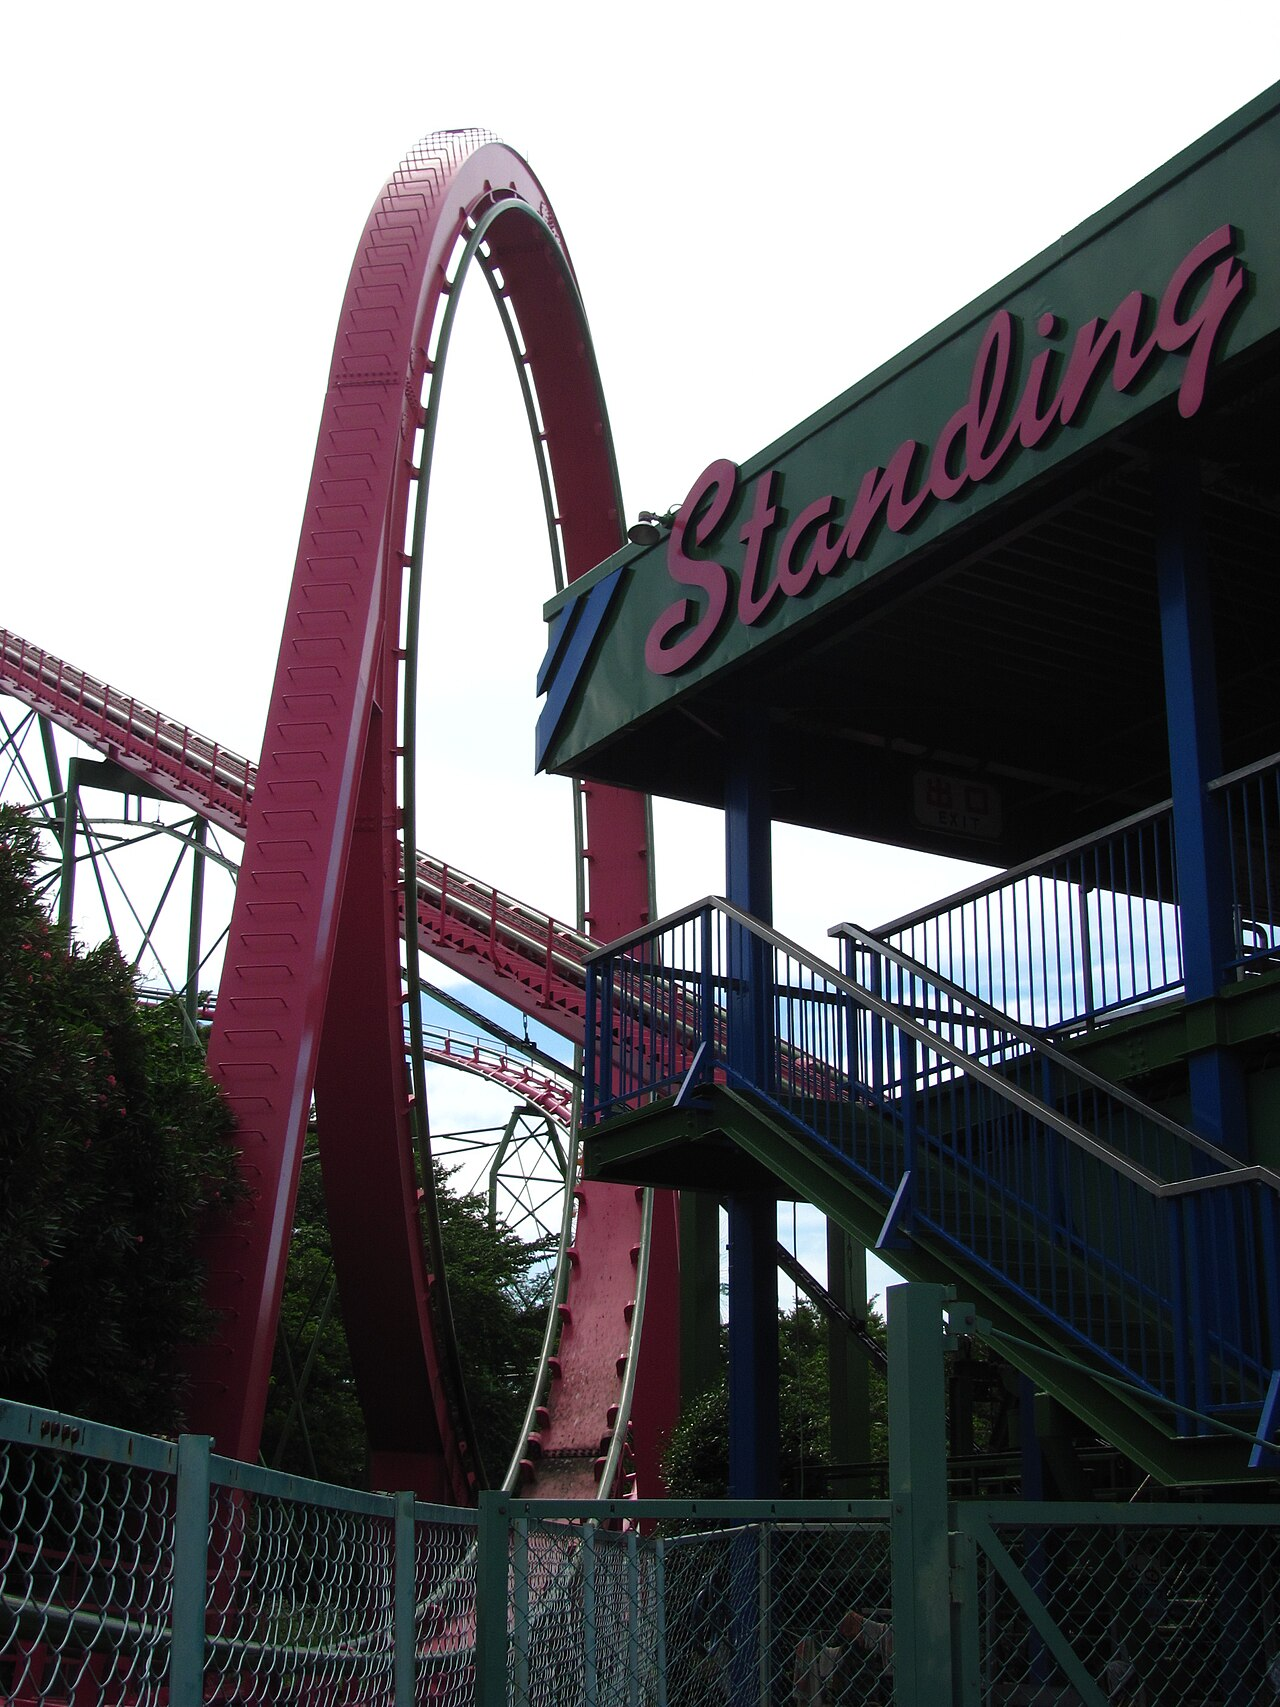
\includegraphics[width=0.38\linewidth]{images/book3/roller-coaster-loop.jpg}

{\small Sebuah loop tegak (Yomiuriland, Tokyo): berbentuk tetes air \omterm{def:b1:optical-instruments:eye}{mata} dan bukan lingkaran, sehingga kelengkungannya terbesar di puncaknya tempat kelajuannya terkecil --- geometri soal akhir pekan. Foto: Jeremy Thompson, CC\ BY\ 2.0.}
\end{omfigure}

\section{Soal: Loop kereta luncur}

\begin{problem}[{Soal akhir pekan --- sebuah kereta memasuki loop tegak
pada sembilan puluh kilometer tiap jam: di mana ia melambat, ke mana
percepatannya menunjuk, berapa $g$ yang dirasakan penumpangnya, dan
mengapa loop modern bukan lingkaran}]
\label{pb:b1:point-kinematics:1}
Sebuah kereta, yang diperlakukan sebagai titik $M$, berjalan pada loop
melingkar tegak berjari-jari $R = \qty{10}{m}$, berpusat $C$.
Kedudukannya diberikan oleh sudut $\theta$ antara $\vect{CM}$ dan garis
tegak ke bawah ($\theta =
0$ di dasarnya, $\pi$ di puncaknya). Gesekan
diabaikan, dan hukum kelajuannya (diturunkan dalam
\cref{ch:b1:work-and-energy}) adalah
\[
v^2 = v_0^2 - 2gR(1 - \cos\theta),
\]
dengan $v_0 = \qty{25}{m/s}$ sebagai kelajuan di dasarnya; $g = \qty{9.81}{m/s^2}$.

\medskip
\noindent\textbf{Bagian I --- Kinematika pada lingkarannya.}
\begin{enumerate}
  \item Dalam \omterm{def:b1:point-kinematics:cylindrical}{koordinat polar} yang berpusat di $C$ (dengan $\vect e_r$
        dari $C$ ke $M$), tuliskan $\vect v$ dan $\vect a$ bagi gerak
        pada lingkarannya.
  \item Kenali vektor Frenet $\vect T$ dan $\vect N$ dalam
        $\vect e_r$ dan $\vect e_\theta$, serta \omterm{def:b1:point-kinematics:frenet}{jari-jari kelengkungannya}.
  \item Hitunglah kelajuannya di puncaknya, dan di titik sampingnya
        $\theta = \pi/2$ dan $3\pi/2$.
  \item Turunkan hukum kelajuannya terhadap waktu untuk menunjukkan
        bahwa \omterm{thm:b1:point-kinematics:frenet}{percepatan tangensialnya} $a_T = -g\sin\theta$. Tafsirkan
        tandanya pada perjalanan naik dan pada perjalanan turun.
  \item Nyatakan \omterm{thm:b1:point-kinematics:frenet}{percepatan normalnya} $a_N(\theta)$ lalu hitunglah di
        dasarnya, di sampingnya dan di puncaknya.
  \item Berikan norma $\vect a$ pada keempat titik itu dan sudut yang
        dibentuknya dengan garis tegak di puncaknya.
  \item Pada titik mana $\vect a$ tegak lurus terhadap $\vect v$? Sejajar?
\end{enumerate}

\medskip
\noindent\textbf{Bagian II --- Laju sudut dan pewaktuannya.}
\begin{enumerate}[resume]
  \item Nyatakan $\dot\theta$ sebagai fungsi $\theta$ lalu hitunglah di
        dasarnya dan di puncaknya.
  \item Tunjukkan bahwa $\ddot\theta = -(g/R)\sin\theta$ (persamaan
        sebuah bandul) lalu berikan komentar.
  \item Sebagai pembanding, hitunglah periode osilasi kecil sebuah
        bandul sederhana sepanjang $R$
        (\cref{ex:b1:units-dimensions:pendulum} telah memberikan
        bentuknya; $k = 2\pi$).
  \item Taksirlah waktu untuk mengelilingi loopnya, dengan memakai
        rata-rata kelajuan pada keempat titik acuannya.
  \item Kelajuan minimum di puncaknya agar keretanya tetap pada
        \omterm{def:b1:point-kinematics:frame}{lintasannya} (bab berikutnya) adalah $\sqrt{gR}$. Apakah syarat
        itu terpenuhi? Berapa $v_0$ minimum yang diperlukan?
\end{enumerate}

\medskip
\noindent\textbf{Bagian III --- Apa yang dirasakan penumpangnya.}
Berat semu tiap satuan massa yang dirasakan seorang penumpang adalah
$\vect a - \vect g$ (diterima saja di sini, diturunkan dalam
\cref{ch:b1:newton-dynamics}); normanya dalam satuan $g$ disebut ``beban-$g$''.
\begin{enumerate}[resume]
  \item Hitunglah beban-$g$ di dasarnya.
  \item Hitunglah di puncaknya, lalu katakan ke arah mana penumpangnya
        tertekan (ke kursinya atau ke pengamannya).
  \item Hitunglah di titik sampingnya.
  \item Penumpang menoleransi sekitar $4g$ untuk waktu singkat. Apakah
        loop ini lolos? Di mana masalahnya?
  \item Tunjukkan bahwa, untuk loop melingkar yang dimasuki tepat cukup
        cepat untuk melewati puncaknya (berat semunya nol di sana),
        beban-$g$ di dasarnya niscaya $6g$, berapa pun $R$-nya.
\end{enumerate}

\medskip
\noindent\textbf{Bagian IV --- Loop klotoid.}
Loop modern berbentuk ``tetes air \omterm{def:b1:optical-instruments:eye}{mata}'': \omterm{def:b1:point-kinematics:frenet}{jari-jari kelengkungannya}
besar di dasarnya dan kecil di puncaknya.
\begin{enumerate}[resume]
  \item Dengan memakai bentuk Frenet $\vect a$, jelaskan mengapa
        mengubah $\rho$ di sepanjang \omterm{def:b1:point-kinematics:frame}{lintasannya} mengubah $a_N$ tanpa
        mengubah hukum kelajuannya (yang hanya bergantung pada
        ketinggiannya).
  \item Pilihlah $\rho_{\text{dasar}}$ agar beban-$g$ di dasarnya $3g$
        dengan $v_0 = \qty{25}{m/s}$.
  \item Di puncaknya, ketinggiannya tetap $2R = \qty{20}{m}$ di atas
        dasarnya. Pilihlah $\rho_{\text{puncak}}$ agar beban-$g$ di sana
        $1.5g$.
  \item Sebuah klotoid berkelengkungan sebanding dengan panjang
        busurnya, $1/\rho = s/A^2$. Menyusuri jalan masuk semacam itu,
        dengan kelajuan yang nyaris tetap, bagaimana $a_N$ tumbuh
        terhadap waktu, dan mengapa hal itu lebih lembut bagi leher
        daripada lingkaran (yang $a_N$-nya melompat di jalan masuknya)?
  \item Sketsalah bentuk loop yang dihasilkannya secara kualitatif lalu
        ringkaslah dalam dua kalimat mengapa ia menggantikan lingkarannya.
\end{enumerate}

\medskip
\noindent\textbf{Bagian V --- Dilihat dari tanah.}
Sebuah \omterm{def:b1:optical-instruments:camera}{kamera} setinggi tanah, \qty{50}{m} dari pusat loopnya pada
bidangnya, mengikuti keretanya.
\begin{enumerate}[resume]
  \item Ketika keretanya berada di puncaknya, bergerak mendatar pada
        \qty{15}{m/s}, dengan laju sudut berapa (rad/s) \omterm{def:b1:optical-instruments:camera}{kameranya} harus
        berputar? (\omterm{def:b1:point-kinematics:cylindrical}{Koordinat polar} dari \omterm{def:b1:optical-instruments:camera}{kameranya}.)
  \item Mengapa \omterm{def:b1:optical-instruments:camera}{kamera} yang berputar dengan laju tetap merupakan
        pengikut yang buruk bagi \omterm{cor:b1:point-kinematics:circular}{gerak melingkar} beraturan?
  \item Ringkaslah pelajaran bab ini dari loopnya: sistem koordinat mana
        yang menjawab pertanyaan yang mana.
\end{enumerate}
\end{problem}
